\graphicspath{{./eighth/img/}} % path to graphics

\section*{Выполнение практической работы}
\addcontentsline{toc}{section}{Выполнение практической работы}
Сервер обрабатывает запросы, поступающие с автоматизированных рабочих мест
с интервалами, распределенными по показательному закону со средним
значением 2 мин. Время обработки
сервером одного запроса распределено по экспоненциальному закону со
средним значением 3 мин. Сервер имеет входной буфер ёмкостью 5 запросов.
Построить имитационную модель для определения математического ожидания
времени и вероятности обработки запросов.
Сервер представляет собой однофазную систему массового обслуживания
разомкнутого типа с ограниченной входной емкостью,
то есть с отказами, и абсолютной надёжностью.\par
Итоговая модель проиллюстрированна на рисунке~\ref{fig:model:res}.

\begin{image}
	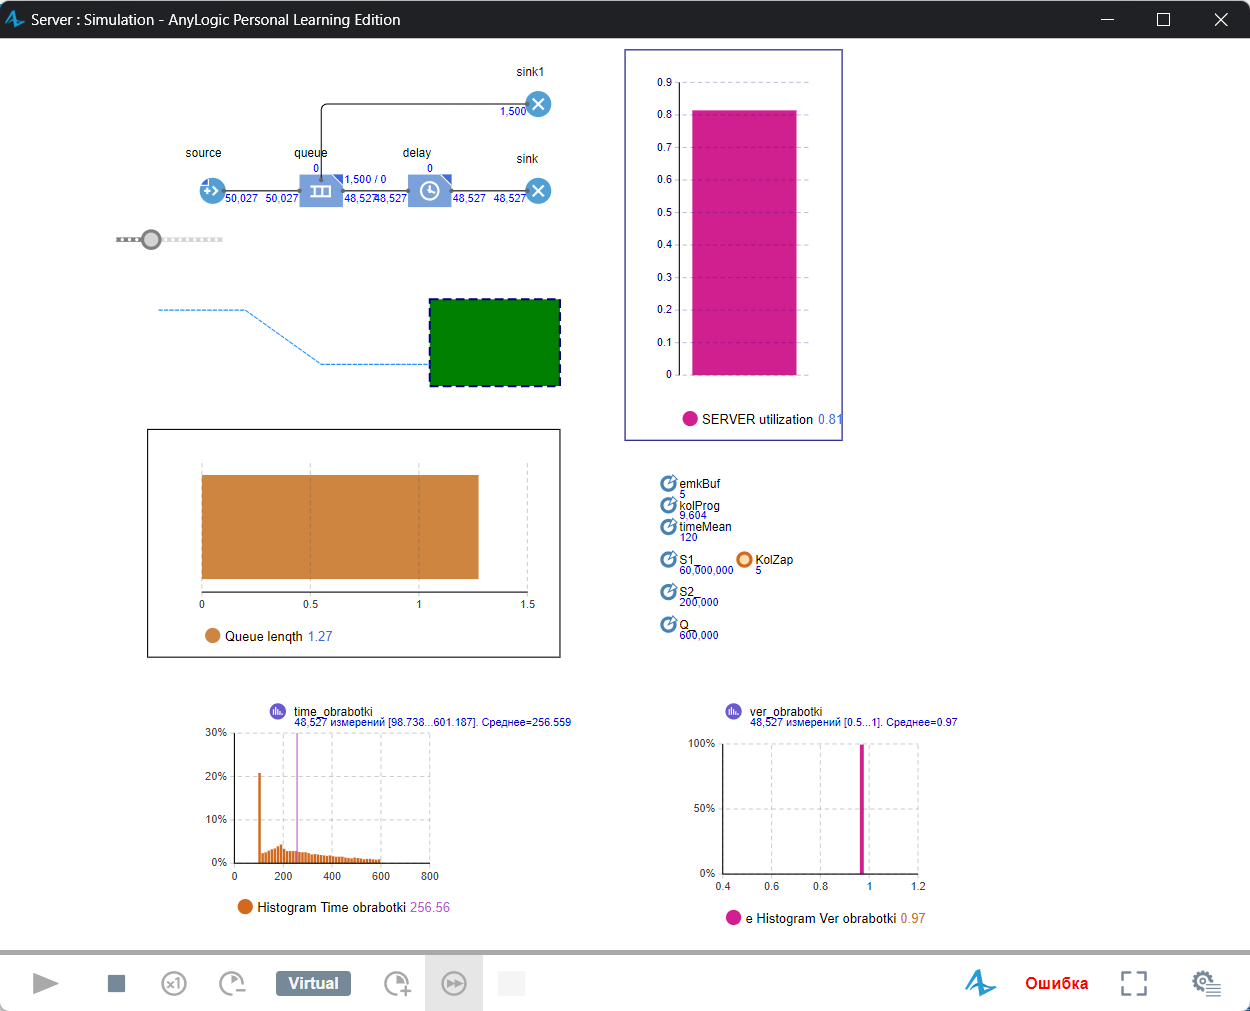
\includegraphics[width=1\textwidth]{2023-05-06_18-02-40}
	\caption{Модель сервера}
	\label{fig:model:res}
\end{image}

\clearpage

\section*{\LARGE Вывод}
\addcontentsline{toc}{section}{Вывод}
В данной практической работе была создана модель сервера.\par
Проведём несколько экспериментов. Будем изменять среднее
время поступления запросов timeMean в предположении, что с течением времени
количество источников запросов будет расти, то
есть timeMean будет уменьшаться. В сторону увеличения будем
изменять ёмкость входного буфера emkBuf и производительность Q\_ сервера.\par
Результаты экспериментов приведены в табл.~\ref{tabl:exp}.

\begin{longtable} {
	|p{0.35\textwidth}
	|p{0.1\textwidth}
	|p{0.13\textwidth}
	|p{0.13\textwidth}
	|p{0.13\textwidth}
	|}
	\caption{\leftline{Показатели функционирования направления связи}}
	\label{tabl:exp}\\
	\hline Показатели & GPSS World & AnyLogic6
		& AnyLogic7 & AnyLogic8 \\ \hline
	\endhead

	\multicolumn{5}{|c|}{1) timeMean = 120, emkBuf = 5} \\ \hline
	Количество обработанных запросов & 29 & 29 & 29 & 5 \\ \hline
	Вероятность обработки запросов & 0,970 & 0,971 & 0,970 & 0,97 \\ \hline
	Среднее время обработки одного запроса & 255,262 & 254,942
		& 255,727 & 256,56 \\ \hline
	Средняя длина очереди запросов к серверу & & 1,254 & 1,261 & 1,27 \\ \hline
	Коэффициент использования сервера & 0,810 & 0,810 & 0,810 & 0,81 \\ \hline
	\multicolumn{5}{|c|}{2) timeMean = 120, emkBuf = 10} \\ \hline
	Количество обработанных запросов & 29 & 30 & 30 & 5 \\ \hline
	Вероятность обработки запросов & 0,995 & 0,995 & 0,995 & 0,99 \\ \hline
	Среднее время обработки одного запроса & 328,328 & 321,540
		& 325,017 & 337,01 \\ \hline
	Средняя длина очереди запросов к серверу & & 1,841 & 1,870 & 1,99 \\ \hline
	Коэффициент использования сервера & 0,833 & 0,831 & 0,831 & 0,84 \\ \hline
	\multicolumn{5}{|c|}{3) timeMean = 40, emkBuf = 5}\\ \hline
	Количество обработанных запросов & 36 & 36 & 36 & 2 \\ \hline
	Вероятность обработки запросов & 0,400 & 0,399 & 0,400 & 0,4 \\ \hline
	Среднее время обработки одного запроса & 1055,335 & 1055,108
		& 554,983 & 555,56 \\ \hline
	Средняя длина очереди запросов к серверу & & 4,552 & 4,550 & 4,56 \\ \hline
	Коэффициент использования сервера & 1,00 & 1,00 & 1,00 & 1,00 \\ \hline
	\multicolumn{5}{|c|}{4) timeMean = 40, emkBuf = 10}\\ \hline
	Количество обработанных запросов & 36 & 36 & 36 & 2 \\ \hline
	Вероятность обработки запросов & 0,399 & 0,399 & 0,400 & 0,400 \\ \hline
	Среднее время обработки одного запроса & 591,860 & 591,304
		& 1054,907 & 1055,23 \\ \hline
	Средняя длина очереди запросов к серверу & & 9,551 & 9,549 & 9,55 \\ \hline
	Коэффициент использования сервера & 1,00 & 1,00 & 1,00 & 1,00 \\ \hline
	\multicolumn{5}{|c|}{5) timeMean = 40, emkBuf = 10, Q\_ = 1000000}\\ \hline
	Количество обработанных запросов & 59 & 60 & 60 & 3 \\ \hline
	Вероятность обработки запросов & 0,666 & 0,665 & 0,667 & 0,66 \\ \hline
	Среднее время обработки одного запроса & 591,860 & 591,304
		& 591,129 & 592,8 \\ \hline
	Средняя длина очереди запросов к серверу & & 8,855 & 8,852 & 8,88 \\ \hline
	Коэффициент использования сервера & 1,00 & 1,00 & 1,00 & 1,00 \\ \hline
	\multicolumn{5}{|c|}{6) timeMean = 40, emkBuf = 15, Q\_ = 2000000}\\ \hline
	Количество обработанных запросов & 90 & 90 & 90 & 5 \\ \hline
	Вероятность обработки запросов & 1,00 & 1,00 & 1,00 & 1,00 \\ \hline
	Среднее время обработки одного запроса & 74,859 & 75,049
		& 75,096 & 75,67 \\ \hline
	Средняя длина очереди запросов к серверу & & 1,096 & 1,128 & 1,15 \\ \hline
	Коэффициент использования сервера & 0,751 & 0,750 & 0,751 & 0,75 \\ \hline
\end{longtable}

Так как роботы выполнялась в бесплатной версии AnyLogic8, было ограничение на
50000 прогонов, что привело к более малому количеству  обработанных запросов,
по сравнению с версиями AnyLogic6 и AnyLogic7.


